% !TeX program = pdflatex
% !BIB program = bibtex
\documentclass[10pt,conference,letterpaper]{IEEEtran}

\usepackage[T1]{fontenc}
\usepackage[utf8]{inputenc}
\usepackage{amsmath,amssymb}
\usepackage{booktabs}
\usepackage{cite}
\usepackage{graphicx}
\usepackage{siunitx}
\usepackage{tabularx}
\usepackage{tikz}
\usetikzlibrary{arrows.meta,positioning}
\usepackage{xurl}
\usepackage[hidelinks,bookmarks=false]{hyperref}
%\usepackage[bookmarks=false]{hyperref}
%\urlstyle{same}
%\sisetup{detect-all=true}
%\hypersetup{
%  pdftitle={UAV Base Station Dense Radio Environment Maps in FR3: Dataset and ML-based modeling},
%  pdfauthor={Guillem Moreno Garcia, Evgenii Vinogradov, Sergi Abadal}
%}

\title{Channel Knowledge Maps for FR3 UAV Base Stations: Dataset and ML-based Modeling}

\author{\IEEEauthorblockN{Guillem Moreno Garcia, Sergi Abadal, Evgenii Vinogradov}
\IEEEauthorblockA{Universitat Polit\`ecnica de Catalunya (UPC), Barcelona, Spain\\
guillem.moreno.garcia@estudiantat.upc.edu}}

\begin{document}
\maketitle

\begin{abstract}
This paper introduces a dense upper mid-band Frequency Range (FR3) Channel Knowledge Map (CKM) dataset for unmanned aerial vehicle (UAV) base stations (UxNBs). It contains 16\,180 CKM samples from 3\,236 urban locations in 66 cities at {7.125}\,{GHz} and UxNB heights of up to \SI{500}{m}. Every 513$\times$513 sample stores the building geometry, the line-of-sight (LOS) state, attenuation, delay spread, angular spread, and variable transmitter height. As a focused first use-case, we propose an interpretable height-aware attenuation model. Its LOS branch combines free-space loss, two-ray term, and compact data-based height/range calibration. Its non-LOS (NLOS) branch combines a COST\,231-Hata basis with local environment-specific linear calibration. The proposed model reaches {1.93}\,{dB} overall root mean square error, with {1.74}\,{dB} in LOS and {3.54}\,{dB} in NLOS on over 500 unique locations in 14 unseen cities (2\,590 samples in total). Its median inference latency is \SI{60.2}{ms} per map. The result provides attenuation data for FR3 UxNB deployments and a physical anchor for future FR3 modeling efforts.
\end{abstract}

\begin{IEEEkeywords}
air-to-ground channel, FR3, channel knowledge map, 6G, radio map, unmanned aerial vehicle.
\end{IEEEkeywords}

\section{Introduction}
Unmanned Aerial Vehicles (UAVs) with an on-board base station (UxNB) are often seen as one of the key enablers of future 6G networks due to their mobility and better Line-of-Sight (LOS) channels~\cite{Vinogradov2018,Geraci2022ntn}. However, UxNB deployment faces challenges such as location optimization and real-time channel state estimation on resource-constrained UxNBs. Environment-aware communication enabled by Channel Knowledge Maps (CKMs) aims to resolve these challenges~\cite{ckmtutorial2024}. A CKM is a site-specific database containing the locations of transmitters and/or receivers, providing location-specific channel knowledge useful to enhance environment-awareness and facilitate channel acquisition or obviate the need for it entirely. Any relevant information can be stored in a CKM, including but not limited to channel gains, multi-path delays/angles, or even the full channel impulse response~\cite{zengx2021ckm}.

CKMs can be obtained via measurements or channel modeling. Measurements provide the most accurate results, but may be cumbersome. The models used for simulating wireless channels range from a fully stochastic to fine-grained deterministic ray-tracing (RT) model depending on the requirements for precision and the geographical scale. Most available CKM datasets~\cite{dataset2212,ckmimagenet2025} rely on RT simulated data. Since RT simulators are known to be resource-demanding, faster learning-based simulation approaches have become popular \cite{Chen2017rem,radiounet2020,pmnet2023, pmnet_icassp2023}. Prediction of dense channel gain maps is commonly approached as an image-to-image regression problem: RadioUNet~\cite{radiounet2020} and PMNet~\cite{pmnet2023, pmnet_icassp2023} systems demonstrate the strength of convolutional encoder--decoder models when city topology and sparse or simulated channels are available. 

Recently, the upper mid-band Frequency Range (FR3, between 7 and 24\,GHz) has started to gain attention as a promising spectrum candidate to enhance both coverage and capacity of 6G networks~\cite{Cui2024}. FR3 offers a balance between the reliable propagation of sub-6\,GHz bands (FR1) and the large bandwidth of millimeter-wave bands (FR2). FR3 is very attractive for UxNB deployments that have better LOS conditions but still must reliably function in Non-LOS (NLOS) scenarios.  To assess and harness the potential of UxNB-enabled networks in FR3, we need accurate channel data in diverse urban environments. Unfortunately, to our knowledge, there are no publicly available UxNB CKM datasets in FR3.

\begin{table}[b]
\vspace{-15pt}
\centering
\caption{Comparison of Different CKM Datasets}
\vspace{-2pt}
\begin{tabular}{@{}c|c|c|c@{}}
\toprule
Properties  & Ours   &  \cite{dataset2212}  &  \cite{ckmimagenet2025} \\ \hline 
Frequency Range & FR3   & FR1 & FR2\\ \hline 
Variable elevated Tx height & yes   & no & no\\ \hline 
Number of Layouts & 3\,236  & 701  & $>10\,000$ \\ \hline 
Size of Sample  & 513$\times$513& 256$\times$256  & 128$\times$128 \\  \hline 
Horizontal Resolution & 1 m & 1 m  & 2 m\\ \hline 
Real Buildings Footprint  & yes   & yes     & yes \\  \hline 
\bottomrule
\end{tabular}
\label{tab:datasets}
\end{table}

\paragraph{Limitations of the existing CKM datasets}
The existing CKM datasets are summarized in Table~\ref{tab:datasets}. It can be seen that the datasets i) contain only FR1 or FR2 channels; ii) do not use UxNB-specific geometries (coverage size and transmitter (Tx) heights); iii) use non-accurate 3D city models. 

\begin{figure*}
\centering
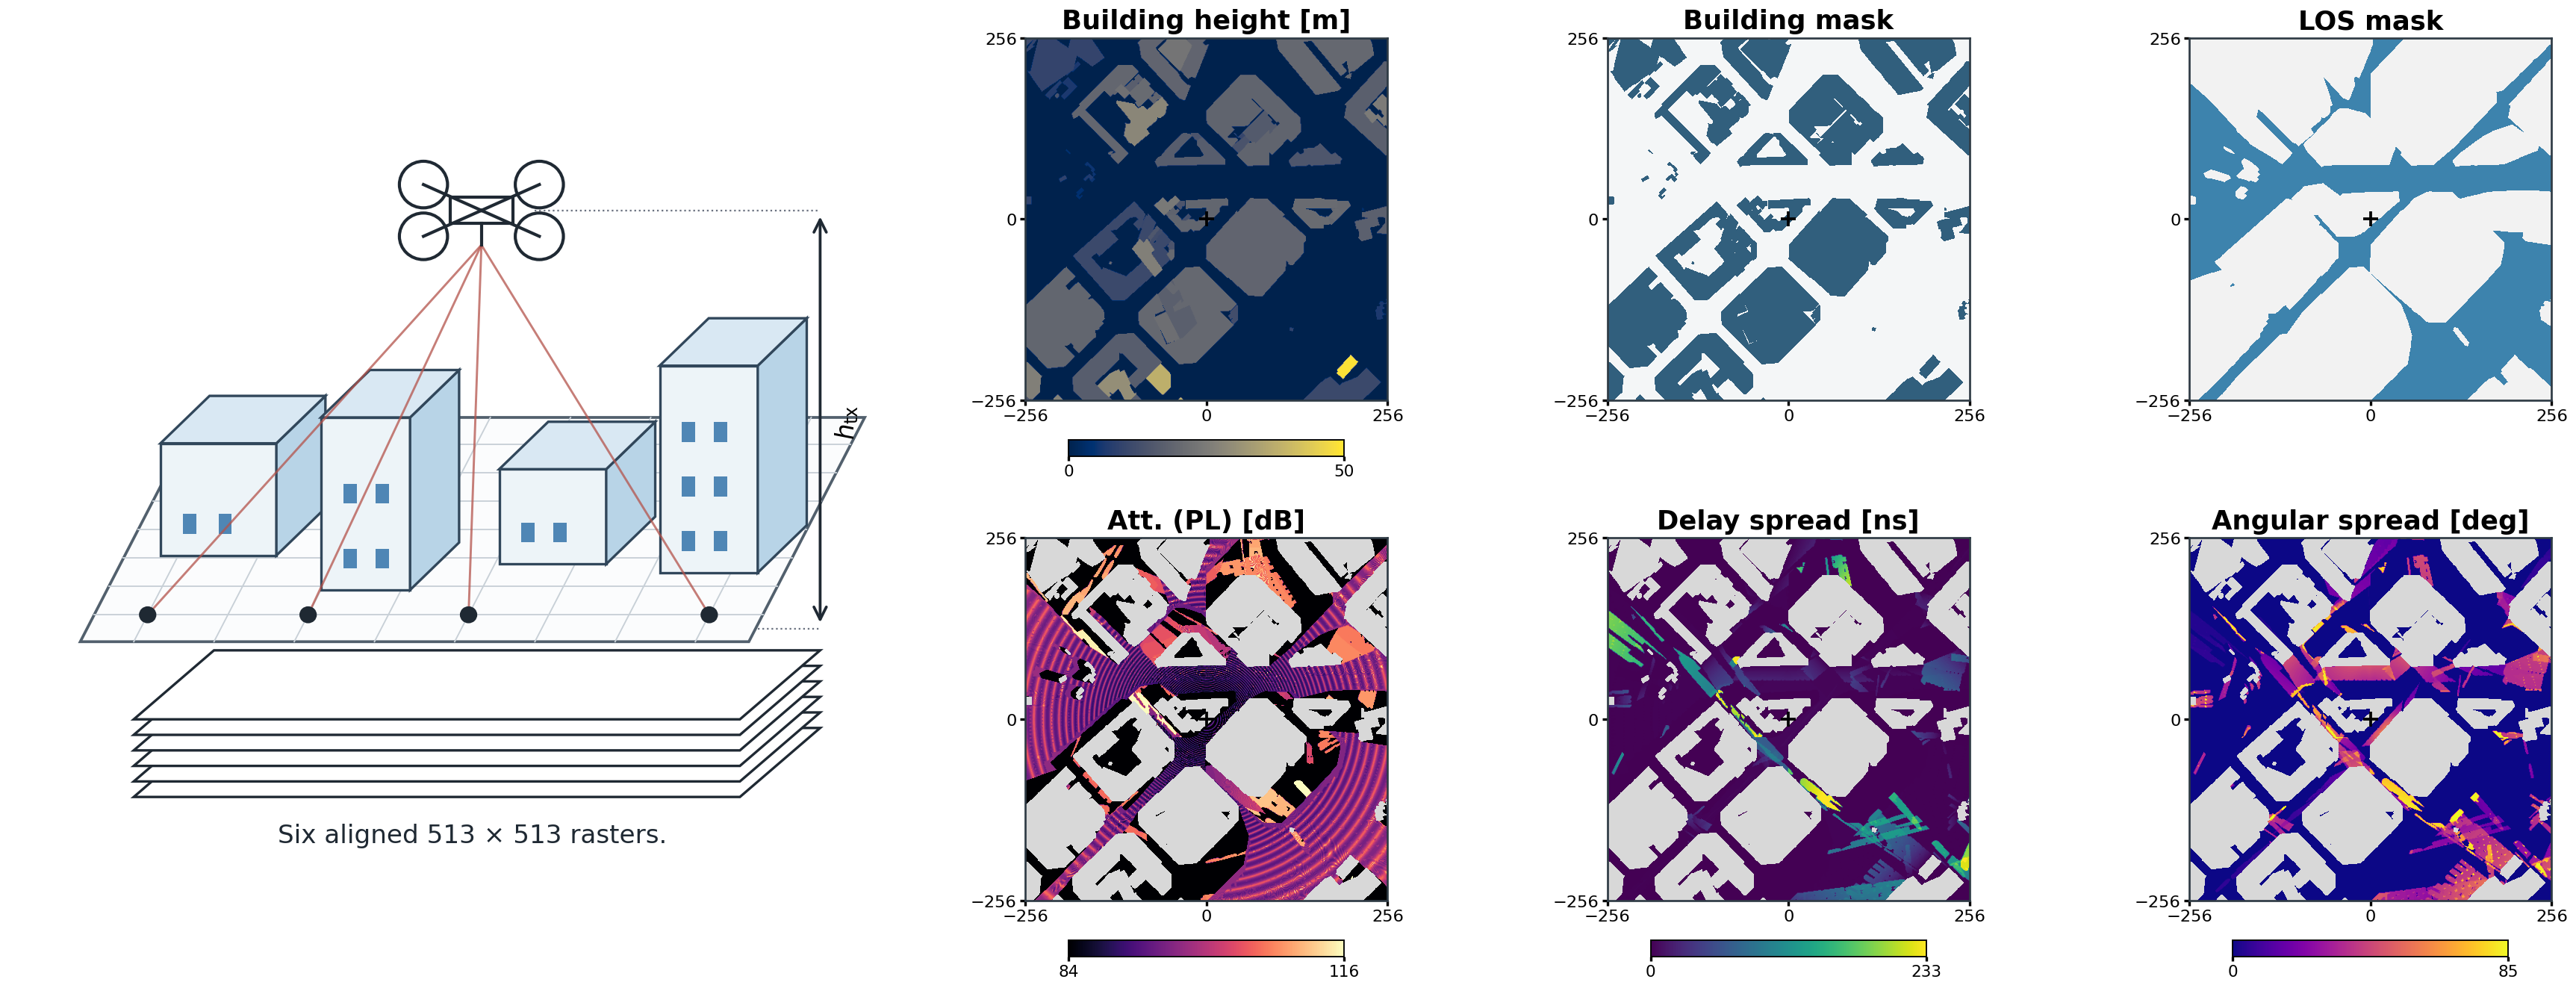
\includegraphics[width=0.85\textwidth]{figures/ckm_dataset_real_sample.png}
\caption{An example of a CKM sample from Barcelona. Left: Links from an elevated UAV base station to ground receivers in a 3D urban topology. Right: The corresponding six aligned $513 \times 513$ channels comprising $L=2$ environmental channels and $F=4$ channel quantities.}
\label{fig:ckm_sample}
\vspace{-8pt}
\end{figure*}

CKM for UxNB should contain information on a typical cell coverage diameter (\SIrange{300}{500}{m}) with a spatial resolution that is capable of capturing important channel variations (20--80 wavelengths) of channel parameters~\cite{saboor26}. Since UxNBs can use heights up to \SI{500}{m}, the resulting channel is very different from terrestrial channels~\cite{khawaja2019survey,Vinogradov2018}. UrbanRadio3D~\cite{radiodiff2025} uses receiver heights up to \SI{20}{m}, but does not provide the continuously variable elevated-transmitter geometry considered here. Moreover, Air-to-Ground (A2G) channel modeling requires accurate information about building height~\cite{vinogradov2026upsim}. The existing datasets use OpenStreetMap (OSM) city layouts. Although OSM contains accurate information about building footprints, critical building height information is only available in less than 10\% of cases~\cite{Bernard2022}.

\paragraph{Limitations of the existing CKM modeling approaches}
Existing learning-based channel map estimation frameworks suffer from several architectural and practical limitations. First, dense attenuation-map prediction is commonly approached via pure image-to-image regression, employing heavy, over-parameterized convolutional networks to rediscover propagation physics (e.g., free-space path loss) independently for every environment. Second, these architectures typically assume fixed terrestrial geometries and fail to reproduce the effect of varying transmitter altitudes typical for UxNB deployments. Finally, pure deep learning approaches struggle with spatial generalization; they often require local fine-tuning when deployed in unseen cities and urban topologies. 

\paragraph{Beyond state-of-the-art contributions}
In this paper, we address these gaps. The main contributions are:
\begin{enumerate}
    \item We introduce an FR3 (7.125 GHz) CKM dataset\footnote{\url{https://doi.org/10.5281/zenodo.21839567}} generated via ray-tracing simulations in 3\,236 city layouts across 66 diverse cities. This dataset relies on complete, global-scale 3D building data~\cite{Che2024globfp,Zhu2025atlas}. UxNB applications are enabled by using Tx heights up to \SI{500}{m} (5 random heights per layout resulting in a total of 16\,180 CKM samples). 
    \item We propose a height-aware channel prediction framework\footnote{\url{https://github.com/unworthyzeus/CKMAttenuationPriors/tree/main}} that explicitly separates LOS and NLOS propagation using local city geometry. By calibrating deterministic baseline models (e.g., free-space path loss, two-ray, COST\,231-Hata) via lightweight regression, the proposed approach achieves highly accurate, zero-shot spatial generalization to completely unseen cities while offering computational speedups. We validate it through city holdout, ablation, and cost comparison.
\end{enumerate}

    
The paper is organized as follows: Section~\ref{sec:ckm_dataset} describes the dataset generation and the 3D urban environment modeling, followed by the proposed height-aware channel prediction framework in Section~\ref{sec:ckm_model}. The performance evaluation and generalization results across diverse city scenarios are presented in Section~\ref{sec:results}, and Section~\ref{sec:conclusions} concludes the paper.

\textbf{Notation:} Boldface uppercase letters $\mathbf{X}$ denote matrices or tensors, while ${X}_{p}$ represents the scalar entry of matrix $\mathbf{X}$ at position $p = (i, j)$. Boldface lowercase letters $\mathbf{x}$ denote vectors, and italic letters $x$ denote scalar variables. The operator $\odot$ represents the Hadamard (element-wise) matrix product, and $\mathbf{x}^\top$ denotes the transpose of vector $\mathbf{x}$.

\section{CKM: Definition and Dataset Description}
\label{sec:ckm_dataset}

An example CKM realization of links from a UAV base station to ground receivers is illustrated in Fig.~\ref{fig:ckm_sample}. In the following, we will use the terms UxNB and transmitter interchangeably.

\subsection{CKM Definition and Mapping Formulation}
\label{sec:ckm_def}
We define a CKM sample as a spatial representation combining environmental channels, channel quantities, and operational metadata. For any given CKM sample $n \in \{1, \dots, N\}$, the propagation environment is represented as a tensor $\mathbf{E}_n \in \mathbf{E} \subset \mathbb{R}^{H \times W \times L}$, where $H$ and $W$ denote the spatial grid dimensions (spanning element indices $1$ to $513$), and $L$ is the number of environmental channels (e.g., building heights, terrain information). The radio propagation characteristics are represented as a channel state tensor $\mathbf{C}_n \in \mathbf{C} \subset \mathbb{R}^{H \times W \times F}$, storing $F$ channel quantities at the receiver grid (e.g., attenuation, multi-path delay spread, angular parameters). Operational metadata (e.g., carrier frequencies, UxNB location information) are defined via a metadata vector $\mathbf{m}_n \in \mathcal{M} \subset \mathbb{R}^K$.

Hence, CKM estimation can be framed as finding a parametric mapping function $\mathbf{\Phi}_{\boldsymbol{\theta}}$:
\begin{equation}
\mathbf{\Phi}_{\boldsymbol{\theta}} : \mathbf{E} \times \mathcal{M} \to \mathbf{C},
\label{eq:mapping_generic}
\end{equation}
where parameters $\boldsymbol{\theta}$ are optimized such that the estimated channel tensor $\widehat{\mathbf{C}}_n = \mathbf{\Phi}_{\boldsymbol{\theta}}(\mathbf{E}_n, \mathbf{m}_n)$ approximates the ground-truth target $\mathbf{C}_n$.

\subsection{The FR3 UxNB CKM Dataset}
\label{sec:dataset_details}
This subsection describes the two environmental input channels, four ray-traced channel quantities, and metadata distributed with each realization.

\subsubsection{3D urban environment modeling ($\mathbf{E}$)}
\label{sec:env_model}
The environmental tensor $\mathbf{E}_n$ in our dataset relies on global-scale 3D building datasets~\cite{Che2024globfp,Zhu2025atlas}. For UxNB deployments, this offers a clear advantage over relying on OSM data popular in literature. OSM is highly valuable for footprint extraction, but height-related tags such as {"height"} and {"building:levels"} are optional and their availability is less than 10\%~\cite{Bernard2022}. By contrast, combining 3D-GloBFP~\cite{Che2024globfp} and GlobalBuildingAtlas~\cite{Zhu2025atlas} provides consistent building height information\footnote{Both datasets claim global coverage but some geographical locations are missing. For example, GlobalBuildingAtlas~\cite{Zhu2025atlas} does not contain the map of Barcelona and some other cities in the EU, while it covers many cities in East Asia missing in 3D-GloBFP~\cite{Che2024globfp}. In this paper, we first searched locations in the more recent GlobalBuildingAtlas and used 3D-GloBFP as the backup.}. This is crucial for UxNBs that depend heavily on deployment height~\cite{Vinogradov2018}.

We extract city layouts of 3\,236 urban locations in 66 diverse cities worldwide to cover a range of propagation topologies (from open low-rise suburbs to dense high-rise downtown areas). Each rasterized environmental map $\mathbf{E}_n$ spans a spatial grid of $H = W = 513$ at a horizontal resolution of $1\text{~m}$. The odd size centers the transmitter, spans offsets from $-256$ to $256$, and captures a wider propagation field than $256\times256$. The $L=2$ environmental channels encode:
\begin{itemize}
    \item Building height profile maps $\mathbf{H}$ indicating building height in meters ($0\text{~m}$ over ground level).
    \item Binary building occupancy masks $\mathbf{B}$ indicating presence of structural obstacles.
\end{itemize}

\subsubsection{Ray-Tracing Channel Simulation ($\mathbf{C}$)}
\label{sec:rt_sim}
High-precision ray-tracing simulations are conducted to generate the spatially consistent channel tensors $\mathbf{C}_n$. To avoid using separate software for 3D model construction (e.g., Blender) and for RT (e.g., Wireless InSite or Sionna), SiteViewer and RT capabilities of MATLAB are used in this work. %Note that MATLAB RT is slightly slower than the mentioned commercial and open solutions~\cite{Zhu2024RT}.

RT simulation parameters are summarized in Table~\ref{tab:rt_params}. The $7.125\text{~GHz}$ frequency was selected since the recent World Radiocommunication Conference (WRC-23) indicated it as the only FR3 test band available in all ITU regions. The $1\text{~m}$ resolution corresponds to 24 wavelengths, ensuring spatial coherence~\cite{saboor26}. The other parameters are selected to be transferable to typical UxNB deployments. The total size of the simulated area is larger than in other datasets~\cite{dataset2212,ckmimagenet2025} and corresponds to an increased UxNB coverage footprint. Moreover, the UxNB is always located in the middle of the layout at elevated heights (10~m to 500~m, sampling 5 heights per location) to reflect the focus on UxNB-centric scenarios. This results in a total dataset size of $N =$ 16\,180 samples ($3\,236 \text{ layouts} \times 5 \text{ Tx heights}$). The receivers are placed at ground level in all non-building coordinates. We use the number of ray interactions from CKM literature~\cite{dataset2212}. The resulting channel state tensors $\mathbf{C}_n$ store radio parameters across $F=4$ channels:
\begin{itemize}
    \item Binary visibility mask $\mathbf{V}$: LOS ($1$) vs. NLOS ($0$) states.
    \item Channel attenuation in dB.
    \item Multi-path root-mean-square (RMS) delay spread in ns.
    \item  Multi-path RMS angular spread in degrees.
\end{itemize}
In-building elements are assigned a value of $0$ in $\mathbf{C}_n$ and should be masked out during training and evaluation.

\subsubsection{Metadata ($\mathbf{m}$)}
\label{sec:metadata}

Because carrier frequency, receiver height, and horizontal transmitter location (fixed at the grid center) are constant across all simulations, the metadata vector $\mathbf{m}_n$ consists of:
\begin{itemize}
    \item Transmitter height $h_{\text{tx}}$ ranging from $10\text{~m}$ to $500\text{~m}$.
    \item Classifying tag mapping the city layout into the closest standard ITU urban topology~\cite{iturp1410} based on building coverage $\alpha$, the density $\beta$ (buildings/km$^2$) as well as the mean building height $\gamma$:
\end{itemize}

    \begin{center}
    \small
    \begin{tabular}{|l|c|c|c|c|}
    \hline
    {Topology} & {Samples} & $\alpha$ & $\beta$ [km$^{-2}$] & $\gamma$ [m] \\ \hline
    Suburban    & 7\,435 & 0.1 & 750 & 8  \\ \hline
    Urban       & 7\,350 & 0.3 & 500 & 15 \\ \hline
    Dense Urban & 1\,395 & 0.5 & 300 & 20 \\ \hline
    \end{tabular}
    \end{center}
The practical $\hat\alpha$, $\hat\beta$, and $\hat\gamma$ differ from the tabular values. Hence, we compute per-topology distances $d=\|\log[(\hat\alpha,\hat\beta,\hat\gamma)/(\alpha,\beta,\gamma)]\|_2$ and choose the smallest. Equal-weight
log-ratios compare relative deviations and prevent the scale of $\beta$ from
dominating. %Note that The urban high-rise prototype $(0.5,300,50)$ is merged into dense urban because only 90 training maps select it.
    
\begin{table}[]
\centering
\caption{Ray Tracing Simulation Parameters}
\label{tab:rt_params}
\begin{tabular}{lc}
\hline
{Parameter} & {Value} \\ \hline
Carrier frequency, $f$ & $7.125\,\text{GHz}$ \\
Antenna model & Isotropic \\
Raster size & $513\times513$ pixels\\
Spatial resolution & $1\,\text{m}$ \\
Ground receiver height, $h_{\text{rx}}$ & $1.5\,\text{m}$ \\
UxNB heights, $h_{\text{tx}}$ & $10\,\text{m}$ to $500\,\text{m}$ \\
UxNB heights per layout & 5 \\
Number of layouts & 3\,236 \\
Total CKM samples, $N$ & 16\,180 \\
Number of ray interactions & 2 \\
\hline
\end{tabular}
\vspace{-0.2cm}
\end{table}

\section{Height-Aware CKM modeling}\label{sec:ckm_model}

\begin{figure}[t]
\centering
\resizebox{\columnwidth}{!}{%
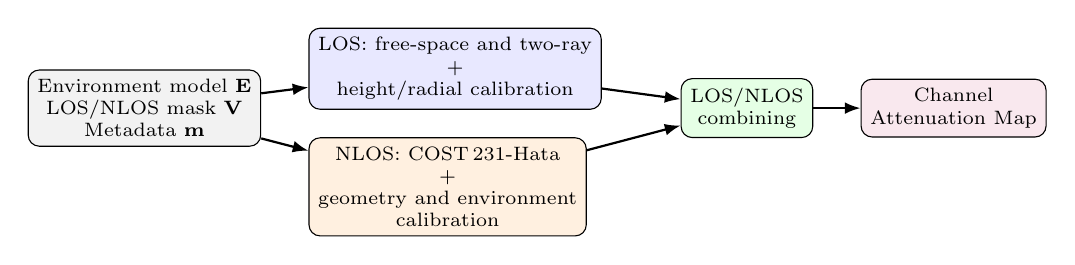
\begin{tikzpicture}[
node distance=5mm and 6mm,
box/.style={draw,rounded corners,align=center,minimum height=7mm,font=\scriptsize},
arr/.style={-{Latex[length=2mm]},thick}]
\node[box,fill=gray!10] (input) {Environment model $\mathbf{E}$ \\ LOS/NLOS mask $\mathbf{V}$\\ Metadata $\mathbf{m}$};
\node[box,fill=blue!9,right=of input,yshift=5mm] (los) {LOS: free-space and two-ray\\+\\height/radial calibration};
\node[box,fill=orange!12,right=of input,yshift=-10mm] (nlos) {NLOS: COST\,231-Hata\\+\\ geometry and environment \\calibration};
\node[box,fill=green!10,right=10mm of los,yshift=-5mm] (switch) {LOS/NLOS \\ combining};
\node[box,fill=purple!9,right=of switch] (out) {Channel \\Attenuation Map};
\draw[arr] (input) -- (los);
\draw[arr] (input) -- (nlos);
\draw[arr] (los) -- (switch);
\draw[arr] (nlos) -- (switch);
\draw[arr] (switch) -- (out);
\end{tikzpicture}}
\caption{The proposed solution uses separate LOS and NLOS propagation models calibrated with training CKM data.}
\label{fig:CKM_model}
\vspace{-0.5cm}
\end{figure}

In this section, we propose a propagation physics-informed CKM attenuation simulator (see Fig.~\ref{fig:CKM_model}). The model implements the attenuation-focused mapping function $\mathbf{\Phi}_{\boldsymbol{\theta}}(\mathbf{E}_n, \mathbf{m}_n)$ by modeling LOS and NLOS attenuation $\Lambda$ separately:
\begin{equation}
\Lambda=\mathbf{V} \odot \Lambda_\text{LOS} + (1-\mathbf{V}) \odot \Lambda_\text{NLOS},
\label{eq:combined}
\end{equation}
where $\odot$ is the element-wise multiplication for masking. 

The proposed LOS attenuation model relies on the free-space and two-ray models corrected with terms learned from the CKM dataset. The proposed NLOS model takes into account the topology characteristics defined by ITU and uses a CKM data-corrected version of the COST\,231-Hata model. Note that we use the visibility mask $\mathbf{V}$ available in the CKM dataset; however, its calculation is straightforward and can be done via RT or shadow projection~\cite{vinogradov2026shadow,vinogradov2026upsim}.

Given the deployment geometry ($h_{\text{tx}}$, $h_{\text{rx}}$, and the fixed horizontal UxNB position), we pre-compute spatial geometry matrices over the $513 \times 513$ grid: horizontal distance $\mathbf{D}_{\text{2D}}$, direct 3D distance $\mathbf{D}_{\text{3D}}$, ground-reflected path length $\mathbf{D}_{\text{GR}}$, and elevation angle $\mathbf{\Theta}_{\text{2D}}$. For any receiver location $p = (i, j)$, the scalar geometric parameters ($d_{\text{2D}}, d_{\text{3D}}, d_{\text{GR}}, \theta$) are indexed directly from these matrices. For notational brevity, we omit the spatial index $p$ in subsequent expressions.

\subsection{Line-of-Sight Branch}
\label{sec:los}
For LOS propagation, the attenuation model combines direct free-space path loss $\Lambda_\text{FSPL}$ with a coherent ground-reflection term $C_{\text{2ray}}$ to capture the two-ray propagation effects. Additionally, the model is calibrated based on CKM data as
\begin{equation}
\Lambda_{\text{LOS}} = \Lambda_\text{FSPL}(d_{\text{3D}}) + C_{\text{2ray}} + \zeta(h_{\text{tx}}) + r(d_{\text{2D}},h_{\text{tx}}),
\label{eq:pl_los}
\end{equation}
where $\zeta(h_{\text{tx}})$ is a height-dependent scalar bias correction and $r(d_{\text{2D}},h_{\text{tx}})$ is a residual component capturing the effects introduced by horizontal distance and transmitter height.

The free-space term follows the Friis distance dependence, while the coherent
correction retains the phase difference between the direct and reflected paths
\cite{rappaport}:
\begin{align}
\Lambda_\text{FSPL}&=20\log_{10}\Big(\frac{4\pi d_\text{3D} f}{c}\Big),\label{eq:fspl}\\
C_{\mathrm{2ray}}&=-20\log_{10}\left|1+\rho(h_{\mathrm{tx}})
\frac{d_{\mathrm{3D}}}{d_{\mathrm{GR}}}
e^{-j[k(d_{\mathrm{GR}}-d_{\mathrm{3D}})+\phi(h_{\mathrm{tx}})]}\right|,
\label{eq:tworay}
\end{align}
where $k$ is the free-space wavenumber, $\rho$ is an effective reflected-field amplitude, and $\phi$ is a fitted phase offset. The calibration terms are obtained in two steps.
Firstly, in each \SI{5}{m} height bin, candidate pairs $(\hat\rho,\hat\phi)$ are evaluated, with $\hat\rho\in\{0,0.05,\ldots,1.5\}$ and 48 uniformly spaced phases $\hat{\phi}$ in $[-\pi,\pi)$. For each pair, the remaining bias is calculated as
\begin{equation}
\hat\zeta(\hat\rho,\hat\phi)=\frac{1}{|B_\text{LOS}|}\sum_{i\in B_\text{LOS}}
\left[y_i-\Lambda_{\text{FSPL},i}-C_{\mathrm{2ray},i}(\hat\rho,\hat\phi)\right],
\label{eq:los-fit}
\end{equation}
where $B_\text{LOS}$ is the set of valid LOS receivers and $y$ is the ground truth attenuation. The triplet $(\hat\zeta,\hat\rho,\hat\phi)$ minimizing the bin Root Mean Square Error (RMSE) is retained.
Secondly, the remaining radial calibration term $r(d_{\text{2D}},h_\text{tx})$ is calculated as the mean of the residual error.


In implementation terms, the LOS calibration is a lookup table that contains height- and distance-dependent $\rho$, $\phi$, $\zeta$, and $r$. Inference linearly interpolates neighboring entries.

\subsection{Non-Line-of-Sight Branch}
\label{sec:nlos}

For shadowed receivers locations, our modeling approach relies on an empirical COST\,231-Hata baseline $\Lambda_C$, augmented by local topographical features derived from the environment map $\mathbf{E}$. The predicted NLOS attenuation is given by:
\begin{equation}
\Lambda_{\text{NLOS}} = \mathbf{x}^\top \hat{\mathbf{w}}_q,
\label{eq:pl_nlos}
\end{equation}
where $\mathbf{x} \in \mathbb{R}^{14}$ is a spatial context feature vector and $\hat{\mathbf{w}}_q$ is the height- and topology-dependent calibrated weight vector.

Evaluated at $f_{\text{MHz}} = 7\,125$\footnote{Since the COST\,231-Hata formulation was designed for sub-3~GHz terrestrial links, we use it as a starting point that needs to be adjusted.}, the term $\Lambda_C$ is computed as:
\begin{align}
\Lambda_C &= 46.3 + 33.9 \log_{10} f_{\text{MHz}} - 13.82 \log_{10} h_{\text{tx}} - a(h_{\text{rx}}) \nonumber \\
&\qquad\quad + \eta(h_{\text{tx}}) \log_{10} (d_{\text{3D}}/1000) + 3,\\ a(h_{\text{rx}}) &= (1.1 \log_{10} f_{\text{MHz}} - 0.7) h_{\text{rx}} - (1.56 \log_{10} f_{\text{MHz}} - 0.8), \\
\eta(h_{\text{tx}}) &= 44.9 - 6.55 \log_{10} h_{\text{tx}}.
\label{eq:cost}
\end{align}

To account for the local environment, we derive 13 contextual features from the building height grid $\mathbf{H}$ and building presence map $\mathbf{B}$ in $\mathbf{E}$. Let $\mathbf{G} = 1 - \mathbf{B}$ be valid outdoor receiver locations and $\mathbf{N} = (1 - \mathbf{V}) \odot \mathbf{G}$ NLOS-ground locations. For $l \in \{15,41\}$, $\mathcal{W}_l(p)$ is the reflect-padded $l\times l$ window centered at receiver $p$ (\SI{1}{m} pixels), and $\mathcal{A}_l[z](p) = l^{-2} \sum_{q \in \mathcal{W}_l(p)} z(q)$.

The full feature vector $\mathbf{x}$ is constructed as:
\begin{equation}
\begin{aligned}
\mathbf x=[&\Lambda_{C},\ell_d,\delta_{15},\delta_{41},h_{15},h_{41},
\delta_{41}\ell_d,\\
&n_{15},n_{41},n_{41}\ell_d,\sigma_{\mathrm{sh}},\theta',
n_{41}\theta',1]^{\top}.
\end{aligned}
\label{eq:nlos-vector}
\end{equation}
where the components represent:
\begin{itemize}
    \item Baseline and Distance: The COST\,231-Hata baseline $\Lambda_C$ and log-radial decay $\ell_d = \ln(1 + d_{\text{2D}})$.
    \item Structural Context: Building density $\delta_l = \mathcal{A}_l[\mathbf{B}]$, normalized building heights $h_l = \mathcal{A}_l[\mathbf{H} \cdot \mathbf{B}] / 90$, and shadowed ground fraction $n_l = \mathcal{A}_l[\mathbf{N}]$ evaluated within local ($l=15$) and regional ($l=41$) windows.
    \item Elevation effects: Normalized path elevation angle $\theta' = \operatorname{clip}(\theta / 90, 0, 1)$, where $\operatorname{clip}(x,a,b)=\min(\max(x,a),b)$, and a deterministic shadowing proxy $\sigma_{\text{sh}} = 2.3197 \left[\max(90 - \theta, 0)\right]^{0.2361}$ as in~\cite{feng2006a2g}.
    \item Interaction Cross-Terms: Density--range $\delta_{41}\ell_d$, blockage--range $n_{41}\ell_d$, and blockage--elevation $n_{41}\theta_n$ interaction terms, alongside the scalar bias unit $1$.
\end{itemize}

The regime weight vectors $\hat{\mathbf{w}}_q$ are calibrated offline using CKM training samples in two steps. Firstly, the scenes are partitioned into $q$ regimes resulting from combinations of the three ITU topologies and three Tx altitude $h_{\text{tx}}$ (nine in total). Altitude regimes are binned into \textit{low} ($h_{\text{tx}} \le 60\text{~m}$), \textit{medium} ($60\text{~m} < h_{\text{tx}} \le 100\text{~m}$), and \textit{high} ($h_{\text{tx}} > 100\text{~m}$). Secondly, for each regime $q$, at most 1\,024 NLoS channel realizations per training sample are fed to the ridge model. For training stability during offline calibration, let $\mathbf{z}_i$ denote the standardized counterpart of the spatial context feature vector $\mathbf{x}_i$ for sample $i$:
    \begin{equation}
    \hat{\mathbf{w}}_q = \arg\min_{\mathbf{w}} \sum_{i \in q} \left( \mathbf{z}_i^\top \mathbf{w} - y_i \right)^2 + 10^{-2} \|\mathbf{w}_{\neg b}\|_2^2,
    \label{eq:nlos-ridge}
    \end{equation}
    where $\mathbf z_i$ contains standardized non-intercept features, and the $L_2$ term penalizes only $\mathbf w_{\neg b}$ while omitting the bias(intercept). %After transforming the coefficients back to raw feature space, the deployed estimate is clipped to the stored attenuation support:
%\begin{equation} \Lambda_{\mathrm{NLOS}}=\operatorname{clip} (\mathbf x^\top\hat{\mathbf w}_q,20,185).\label{eq:nlos-output} \end{equation}







\section{Experiment}\label{sec:results}
\begin{figure}[!t]
\centering
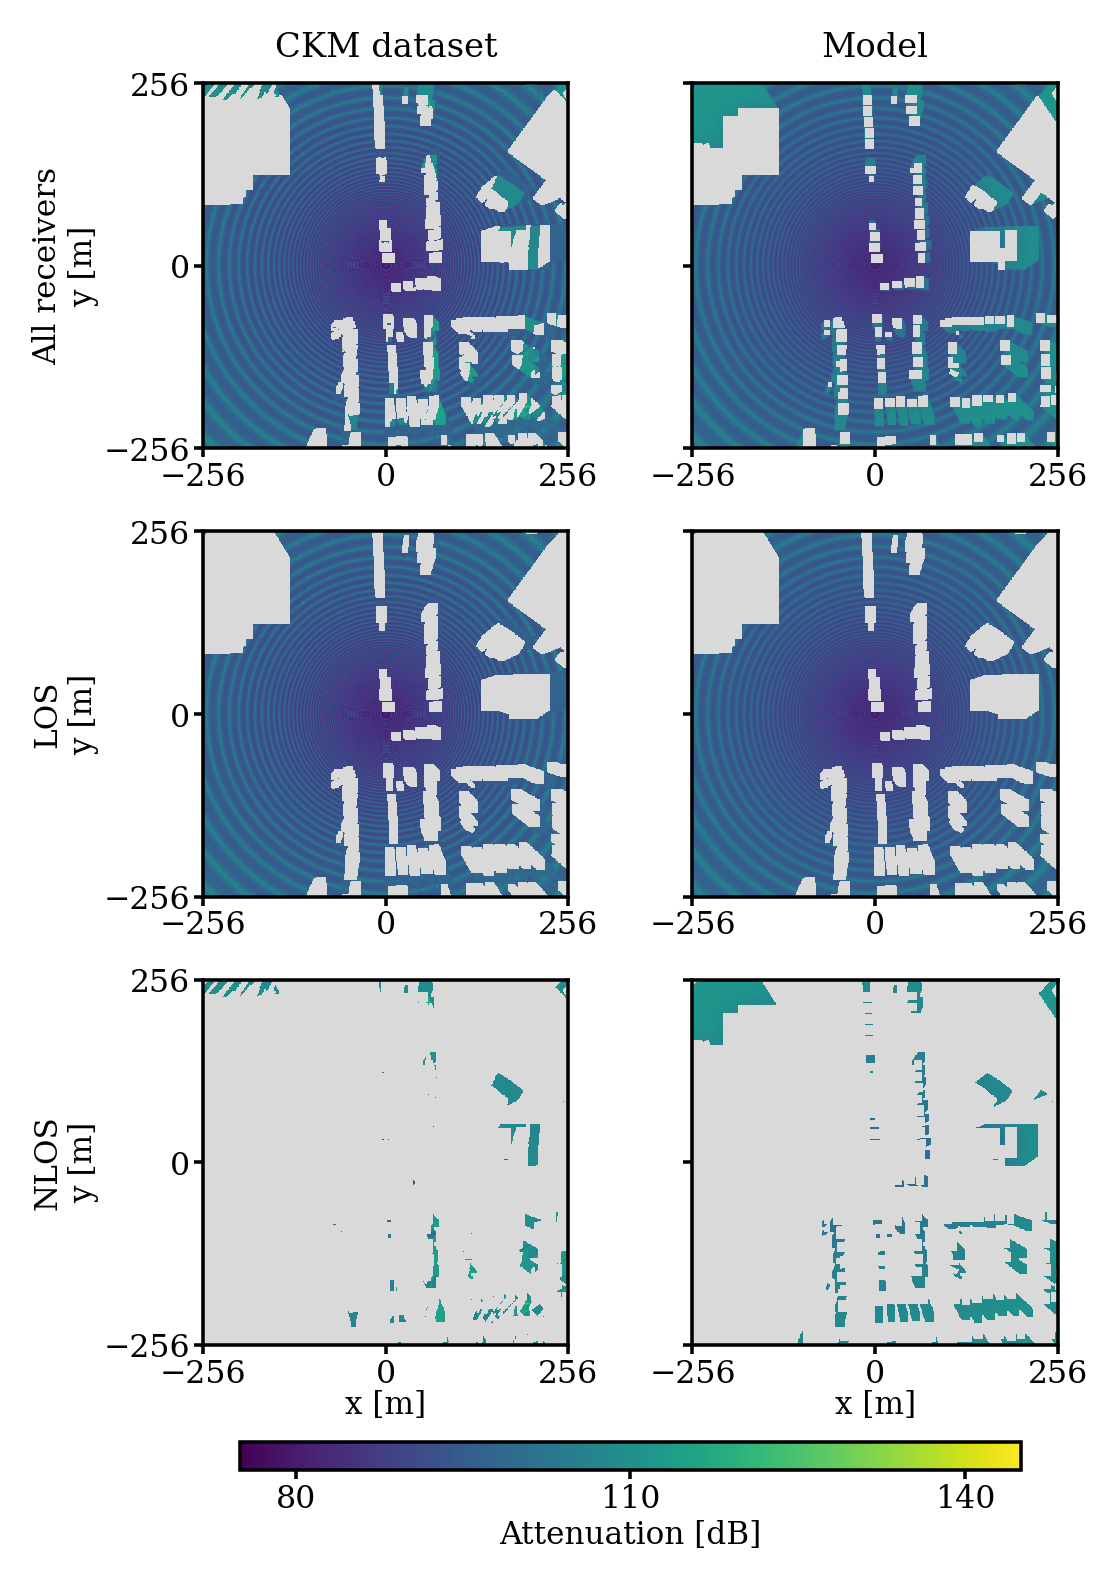
\includegraphics[width=0.8\columnwidth]{figures/nlos_heldout_example.png}
\caption{An example from Vancouver
(``sample\_15262'', $h_{\mathrm{tx}}=${50.30}\,{m}, Dense urban topology, low-transmitter regime). 
The model reproduces attenuation over the unseen layout with {2.18}\,{dB} RMSE. The sample contains 119\,180 LOS and 25\,607 NLOS channels, modeled with {2.10}\,{dB} and {2.52}\,{dB} RMSE. }
\label{fig:output_example}
\vspace{-0.3cm}
\end{figure}

\subsection{Experimental Setup and Evaluation Protocol}
The dataset split contains 10\,840 samples from 37 training cities, 2\,750 samples from 15 validation cities, and 2\,590 samples from 14 final test cities. No city is moved between these partitions to ensure strict spatial generalization. Training procedures described in Section~\ref{sec:ckm_model} use only training cities, where all nine topology and height regimes are fitted on the 10\,840 CKM training samples. The validation subset is reserved for development checks and component ablation. Final performance results use the unseen 14-city test subset.

After excluding building interiors and outdoor channels lacking valid ray-tracing targets, the test dataset evaluates over $4.23 \times 10^8$ ground receivers. Of these, only $7.4\%$ are in NLOS states due to the elevated UxNB geometry. Although the element-weighted overall score is therefore LOS-dominated, 424 of the 2\,590 test maps contain more than $25\%$ NLOS receivers, motivating our separate regime-specific evaluations. An example of the model output can be seen in Fig.~\ref{fig:output_example}.

\subsection{Prediction Accuracy and Height Generalization}
The prediction performance on the unseen test cities across different ITU topologies is summarized in Table~\ref{tab:itu-topology}. Overall, the proposed simulator achieves a global RMSE of \SI{1.93}{dB} (\SI{1.74}{dB} for LOS and \SI{3.54}{dB} for NLOS). While Suburban topology exhibits the lowest total error of \SI{1.70}{dB}, Dense Urban layouts present a harsher NLOS environment with a higher error of \SI{4.13}{dB}. Per-city RMSE ranges from \SI{1.61}{dB} in Halifax to \SI{2.59}{dB} in Osaka, with an unweighted 14-city mean of \SI{1.98}{dB}. The fitted coefficient vectors also change substantially across the ITU topologies, so one global set of slopes would mix distinct relationships. These observations further validate the need for regime calibrations by topology.


Table~\ref{tab:itu-topology} also breaks down the final test error by UxNB altitude regimes. As altitude increases from \SI{10}{m} to \SI{500}{m}, the overall RMSE decreases monotonically from \SI{2.14}{dB} to \SI{1.71}{dB}. This aligns with the observations that higher-altitude channels are usually more stable and predictable~\cite{Vinogradov2018,khawaja2019survey}.


\begin{table}
\centering
\caption{RMSE (in decibels) by ITU topology}
\label{tab:itu-topology}
\scriptsize
\begin{tabular}{lcccc}
\toprule
Topology  & Overall & LOS & NLOS & Test Samples \\
\midrule
Suburban & 1.70 & 1.60 & 3.16 & 1\,455\\
Urban & 2.30 & 2.00 & 3.65 & 940\\
Dense urban & 2.57 & 2.11 & 4.13 & 195\\
\midrule
\midrule
UxNB height & Overall & LOS & NLOS & Test samples \\
\midrule
Low ($h_{\mathrm{tx}}\le\SI{60}{m}$) & 2.14 & 1.79 & 3.75 & 899 \\
Medium ($\SI{60}{m}<h_{\mathrm{tx}}\le\SI{100}{m}$) & 1.97 & 1.77 & 3.51 & 773 \\
High ($h_{\mathrm{tx}}>\SI{100}{m}$) & 1.71 & 1.67 & 2.76 & 918 \\
\midrule
All topologies and heights & 1.93 & 1.74 & 3.54 & 2\,590 \\
\bottomrule
\vspace{-0.6cm}
\end{tabular}
\end{table}

\begin{table}[t]
\centering
\caption{Comparison with Data-Driven Baseline}
\label{tab:accuracy-context}
\scriptsize
\setlength{\tabcolsep}{4pt}
\begin{tabular}{llccc}
\toprule
Method & Type/Grid & Overall & LOS & NLOS \\
\midrule
{Proposed} & Regime calibrated / $513\times513$ & {1.93} & {1.74} & 3.54 \\
GMM U-Net & Neural Baseline / $513\times513$  & 4.36 & 4.43 & {3.34} \\
\bottomrule
\vspace{-0.6cm}
\end{tabular}
\end{table}

To assess the performance of pure end-to-end deep learning on this benchmark, we evaluate a neural baseline (GMM U-Net) utilizing a height-conditioned mixture head and U-Net decoder, trained with the same training split and evaluated on the same 2\,590 test maps and masks. As shown in Table~\ref{tab:accuracy-context}, the proposed model achieves significantly lower global (\SI{1.93}{dB} vs. \SI{4.36}{dB}) and LOS errors (\SI{1.74}{dB} vs. \SI{4.43}{dB}), demonstrating that our LOS model provides superior stability over the purely data-driven approach. Conversely, the lower NLOS error of the GMM U-Net (\SI{3.34}{dB}) indicates that distribution-aware neural heads are well-suited for modeling multipath-dominated NLOS channels.

Published CKM and radio map models are designed under fundamentally different conditions (frequencies, heights, generated outputs) and cannot be directly ranked against our $513 \times 513$ aerial dataset. For scale context, terrestrial model RadioUNet~\cite{radiounet2020} reports RMSEs of \SI{1.60}{dB} on fixed-height $256 \times 256$ RadioMapSeer grids; diffusion-based models such as TSRDiff~\cite{tsrdiff2025} achieve \SI{3.62}{dB} under sparse target sampling; and Gaussian process approaches like RO-HMTGP~\cite{rohmtgp2025} report \SI{4.19}{dB}--\SI{6.00}{dB} on empirical RSRP data. The \SI{1.93}{dB} error of our proposed model shows strong prediction accuracy for larger areas with variable UxNB transmitter altitudes.

\subsection{Ablation Study}
On frozen test data, coherent reflection lowers raw free-space LOS RMSE from \SI{3.99}{dB} to \SI{1.74}{dB}; fitted coefficients plus topology/height calibration lower raw COST\,231-Hata NLOS RMSE from \SI{25.01}{dB} to \SI{3.54}{dB}.

Recalibrated trial-and-error tests selected an eight-coefficient model using 41-pixel morphology that preserves over 90\% of the complete model's error reduction over one global NLOS constant on test; intermediate variants are omitted.


\subsection{Computational Complexity}
Table~\ref{tab:compute} reports same-CPU medians on an AMD Ryzen 5 5600X with GPU disabled. Neural rows use 10 warm-ups and 50 timed passes; the proposed row uses 100 maps, supplied visibility, and excludes file I/O.

\begin{table}[!t]
\centering
\caption{Computational context; reported CPU rows use the same CPU.}
\label{tab:compute}
\scriptsize
\setlength{\tabcolsep}{2.2pt}
\begin{tabular}{@{}lcccc@{}}
\toprule
Method & Grid & Stored scalars & Counted MACs/map & CPU [s] \\
\midrule
Proposed & $513\times513$ & 66.8k+126 & 3.684M$^\ast$ & 0.0602 \\
RadioUNet~\cite{radiounet2020} & $256\times256$ & 13.27M & 12.73G & 0.1339 \\
PMNet~\cite{pmnet2023} & $256\times256$ & 33.34M & 52.71G & 0.4042 \\
SSL-Radio~\cite{sslradio2025} & $256\times256$ & $\approx$15.4--20.4M & $\approx$16.9--21.9G$^\dagger$ & -- \\
MATLAB RT & $513\times513$ & -- & -- & 102.289 \\
\bottomrule
\end{tabular}
\parbox{\columnwidth}{\scriptsize State: 66.8k LOS lookups + 126 NLOS coefficients. $^\ast$Full-grid NLOS dot product only; feature/LOS operations are excluded from MACs but included in time. $^\dagger$SSL-Radio estimate from published layers. RT is a five-layout median with visibility and three channel outputs; timings are orientative and not directly comparable.}
\end{table}

\section{Conclusions}\label{sec:conclusions}
This paper introduced a dense FR3 (7.125 GHz) UAV CKM dataset providing path loss, delay spread, angular spread, and geometric visibility across 16\,180 simulated samples from 66 global cities. Using this dataset, we proposed a computationally efficient, height-aware channel attenuation prediction framework. By relying on conventional models calibrated on the dataset, the model generates highly accurate channel and can generalize to unseen city layouts. The proposed simulator achieves an overall test RMSE of \SI{1.93}{dB} and executes faster than state-of-the-art models, offering a practical, high-performance solution for 6G UxNB deployments.

\bibliographystyle{IEEEtran}
\bibliography{references}

\end{document}
